\setcounter{secnumdepth}{1}
\renewcommand{\chaptername}{Rozdział}
%============================================================================================================================
%							 						Fabuła
%============================================================================================================================
\chapter{Wprowadzenie} 

\section{Fabuła}
\lhead{Rozdział 1. \emph{Fabuła}}

Celem gracza będzie przebiec jak największy dystans. Będzie to bieg astronauty przez obcą planetę na której musi zbierać bańki z tlenem oraz omijać przeszkody żeby nie zginąć. Przeszkodami takimi będą meteoryty zmniejszające poziom życia. Astronauta podczas gry będzie cały czas biec do przodu,zwalniając jedynie w przypadku niskiego poziomu życia.

\begin{wrapfigure}{left}{0.5\textwidth}
\begin{center}

\includegraphics[width=120px]{./Pictures/astro.jpg}
\end{center}
\caption{Postać astronauty }
\label{Etykieta}
\end{wrapfigure}

Poziom życia będzie ciągle spadał, i bańki z tlenem będą go zwiększać. 
Gracz będzie miał możliwość podskakiwania astronautą oraz wznoszenia się nim do góry Sporadycznie na mapie będą się pokazywać bonusy który astronauta będzie mógł zebrać (maksymalnie 3 naraz) i wykorzystać później do uzupełnienia ilości życia. Taki bonus będzie dawał także nieśmiertelność przez kilka sekund, wtedy to na brzegach ekranu pojawi się charakterystyczna obwódka. Kiedy gracz zakończy grę, wtedy jego wynik, czyli ilość przebytych metrów zapisywany będzie na liście 10 najlepszych wyników. Wyniki te będą zapisywane w osobnym pliku na dysku, tak żeby dane nie zostały stracone po wyłączeniu aplikacji. Listę najlepszych wyników będzie można obejrzeć wybierając z głównego menu pozycje „highscore”. Ze względu na fabułę z biegnącym
astronautą, oraz osadzenie zdarzeń na obcej planecie, gra została nazwa „Astro Rush”.


%============================================================================================================================
%							 						 Grafika
%============================================================================================================================
\section{Grafika}
\lhead{Rozdział 1. \emph{Grafika}}

Grafika w grze będzie się opierać o tzw. sprite. Technika ta polega na tworzeniu animacji, bądź też rysowania dużych obrazów z serii małych obrazków
które zazwyczaj są fragmentami jednej grafiki. Poszczególne klatki animacji biegu astronauty przedstawia na rysunek 2.

\begin{figure}[h]
    \centering
    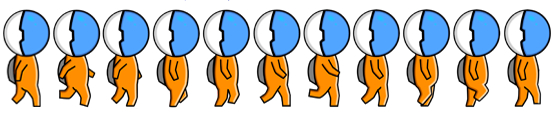
\includegraphics[width=0.8\textwidth,natwidth=410,natheight=142]{./Pictures/astroRun.jpg}
    \caption{Animacja biegu astronauty}
\end{figure}

Wszystkie animacje w grze są przechowywane w jednym głównym pliku „atlas.png”. Skąd wyświetlany jest tylko fragment odpowiadający danemu sprite-owi.
Po upływie określonego czasu następuje przejście do następnej klatki animacji, czyli zazwyczaj przesuniecie współrzędnej X o szerokość obrazka. W tym
algorytmie współrzędna Y nie zmienia się. Cały algorytm wyświetlania animacji opartej przestawia schemat 1.
Warto tutaj wspomnieć o układzie współrzędnych jaki jest używany w bibliotece SDL. Otóż punkt początkowy (0,0) znajduje się w lewym górnym
rogu, prawy górny wierzchołek to ( szerokośćokna, 0 ), natomiast lewy dolny to : (0, wysokość okna ). Grafika na potrzeby gry została częściowo
stworzona w edytorze grafiki wektorowej Inkscape, który oparty jest na licencji GPL i działa pod takimi systemami operacyjnymi jak np. Windows, Linux.
Narysowanie części obrazków jako grafiki wektorowej pozwoliło zachować pełną skalowalność w dalszym procesie tworzenia grafiki. Utworzone grafiki
wektorowe były składane i poprawiane w Adobe Photoshop – bardzo rozbudowanej aplikacji do obróbki grafiki rastrowej. Photoshop jest aplikacją płatną,
jednak istnieje możliwość użycia 30 dniowej wersji Trial, co też zostało zrobione podczas tworzenia gry. W atlasie grafiki znalazły się także ikony z
kolekcji „Hand drawn icon set” które autor opublikował w internecie  na darmowej licencji.

\begin{figure}[h]
    \centering
    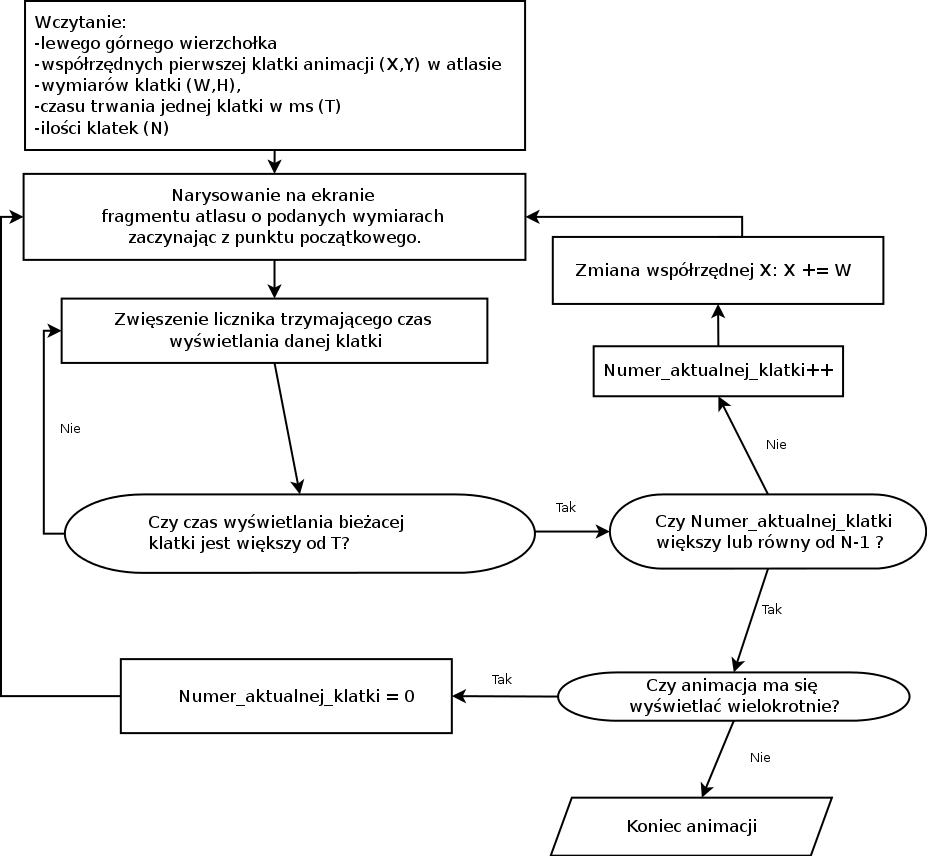
\includegraphics[width=0.8\textwidth,natwidth=410,natheight=142]{./Pictures/sprite_algorytm.png}
    \caption{Schemat wyświetlania animacji opartej o sprite}
\end{figure}


%============================================================================================================================
%							 						Eclipse
%============================================================================================================================
\section{Użyte narzędzia}

\lhead{Rozdział 1. \emph{Użyte narzędzia}}
\subsection{Eclipse}
Środowiskiem w którym będzie powstawać aplikacja będzie Eclipse IDE. Znane jest ono przede wszystkim jako bardzo dobre narzędzie do pisania aplikacji
w Javie, ale dzięki doinstalowaniu wtyczki CDT (C/C++ Development tooling) można w nim rozwijać projekt w języku C++. Eclipse posiada integracje z
wieloma przydatnymi narzędziami, które czasami bardzo upraszczają życie programiście. Przy tworzeniu Astro Rush były wykorzystane:
-Integracja Eclipse z debuggerem. W tym przypadku znany konsolowy gdb.
Najbardziej przydatna okazała się tutaj możliwość zatrzymania programu na breakpoincie oraz sprawdzenie stosu wywołań.
-Integracja z make, co zostanie omówione w kolejnym podrozdziale
-Możliwość doinstalowania kolejnych wtyczek. Przy tworzeniu przydatna
okazała się wtyczka aplikacji Valgrind jako narzędzie do wykrywania wycieków pamięci, oraz integracja z aplikacją Perf. Jest to profiler który
pokazuje statystyki odnośnie tego które wywołania metod trwają najdłużej. Profilowanie okazało się pomocne podczas refactoringu w ramach którego
została przeprowadzona optymalizacja wydajności.


%============================================================================================================================
%							 							Make
%============================================================================================================================
\subsection{Make}
Eclipse jako platforma programistyczna dedykowany jest językowi Java, a kolejne wtyczki pozwalające pisać w innych językach to tylko rozszerzenie tego
środowiska Javy. Eclipse z wtyczką do języka C++ może używać programu Make, który automatyzuje budowanie projektu składającego się z wielu plików.  
Zostało to wykorzystane w projekcie. Ogromnym plusem takiego rozwiązania jest to żeby zbudować aplikacje nie potrzeba ściągać Eclipse-a, ale wystarczy
make, który zajmuje niewiele miejsca na dysku i jest wieloplatformowy. Dodatkowo bardzo łatwo się go instaluje w większości dystrybucji Linuksa. Make
korzysta z pliku reguł domyślnie o nazwie „makefile”. Taki plik dla omawianej gry wygląda następująco:

\begingroup
\fontsize{10pt}{12pt}\selectfont
\begin{verbatim}  
CXX = g++
CFLAGS = -Wall -ansi -pedantic -g -std=c++0x -Wall -I ./include -O0 -c

# flagi linkera
LIBS = -lGL -lGLU -lSDL -lSDL_mixer -lSDL_ttf -lSDL_image -lluabind -llua5.1

# lista plikow źródłowych do kompilacji
SOURCES = src/main.cpp src/App.cpp src/Property.cpp src/Resource.cpp 

# jak maja się nazywać skompilowanie pliki cpp
OBJECTS=$(SOURCES:.cpp=.o)

# nazwa pliku wynikowego
EXECUTABLE = AstroRush.bin

# domyslny cel dla wywolania make bez argumentu, czyli zbudowanie projektu
all: $(SOURCES) $(EXECUTABLE)

# linkowanie aplikacji
$(EXECUTABLE): $(OBJECTS)
	 @echo "\n ---- Linkowanie ---- "
	$(CC) $(OBJECTS) -o $(EXECUTABLE) $(LIBS)

#kompilowanie plikow cpp
.cpp.o:
	 @$(CXX) $(CFLAGS) $< -o $@

# czyszczenie aplikacji przed zbudowaniem  
clean:
	rm -rf ./src/*.o
	rm ./AstroRush.bin 
    \end{verbatim}  
\endgroup

Domyślne wywołanie make bez żadnych parametrów spowoduje zawsze uruchomienie domyślnego celu budowania: all. Możliwe jest definiowania dowolnej ilości
celów budowania w jednym makefile-u. W grze został dodany również cel do czyszczenia gry z wszystkich skompilowanych źródeł oraz zlinkowanej
aplikacji, co okazuje się przydatne kiedy występuje potrzeba przebudowania projektu, bowiem make sprawdza czasy ostatniej modyfikacji  plików tzw.
timestampy i kompiluje tylko te źródła które uległy zmianie od ostatniej kompilacji.
	W napisanym na potrzeby gry pliku „makefile” widać że w plikach makefile można definiować swoje własne zmienne, tutaj na przykład zmienną są
flagi linkera, kompilatora, oraz lista plików źródłowych z katalogu src. Tak napisany makefile jest bardzo uniwersalny i kolejne nowe pliki wymagają
jedynie dopisania ich na listę źródeł. Ewentualnie podczas kompilacji w systemie w którym w zmiennej środowiskowej nie ma kompilatora g++ można tutaj
podać ścieżkę gdzie ten kompilator się znajduje.
	Budowanie aplikacji poprzez make bądź też podobne narzędzie o nazwie cmake jest wyjątkowo popularne w systemie Linuks i projektach napisanych
w języku C/C++. Make jest nawet wykorzystywany do budowania jądra Linuksa, które składa się z milionów linii kodu ( wersja 3.2 to w przybliżeniu 15
mln ) oraz setek plików, gdzie nie wszystkie muszą być skompilowane, a przy rekompilacji kompilowane są tylko te które uległy zmianie, dzięki czemu
oszczędność czasu przy kompilacji jest znacząca.


%============================================================================================================================
%														Git
%============================================================================================================================
\subsection{Git}
Projekt Astro Rush nie wydaje się zbyt duży biorąc pod uwagę fakt że nie przekroczył 10 tysięcy linii kodu. Jednak zawsze warto mieć jakąś kopie na
repozytorium oraz ewentualnie możliwość poprzez historie  zmian przywrócenie jakiś fragmentów kodu. Narzędziem które okazało się tutaj pomocne jest
rozproszony system kontroli wersji – git. Darmowe oprogramowanie stworzone przez Linusa Torvaldsa do zarządzania kodem jądra Linuksa. Git jest również
narzędziem wieloplatformowym, chodź pod systemem Windows jest on wolniejszy niż na Linuksie. Przy tworzeniu aplikacji został wykorzystany serwis
hostujący gita: https://github.com/. Hosting dla aplikacji open source jest darmowy, jednak w takim przypadku repozytorium z kodem jest publiczne.
Warto wspomnieć o tym że serwis github mimo tego że powstał dość nie dawno bo w 2008, ma już 2 miliony repozytoriów.
	Podczas tworzenia aplikacji została wykorzystana wtyczka do eclipse która pozwala w łatwy sposób synchronizować projekt który znajduje się na
dysku lokalnie z tym co jest na repozytorium, oraz wysyłanie zmian na serwer.


\section{OpenGL jako silnik grafiki}
\lhead{Rozdział 1. \emph{OpenGL jako silnik grafiki}}

%============================================================================================================================
%											 Czym jest OpenGL
%============================================================================================================================
\subsection{Czym jest OpenGL}
Open Graphics Library (w skrócie OpenGL) jest niskopoziomową biblioteką  graficzną 3D. Kompatybilny jest on z większością liczących się systemów
operacyjnych, został on także zaimplemtowany na urządzeniach mobilnych, przykładem może być tutaj JOGL, czyli Java-owa wersja OpenGL-a której można
używać na urządzeniach z systemem Android. OpenGL jest często wykorzystywany jako podstawowe API przy tworzeniu silników do gier 3D przykładem może
być tutaj choćby nawet silnik ID tech znany min. z serii gier Quake . Mimo że OpenGL jest przystosowany do pracy z grafiką trójwymiarową to doskonale
można go wykorzystać do grafiki 2D, tak jak to miało miejsce w grze Astro Rush. OpenGL posłużył do wyświetlania tekstur na ekranie, co odbywało się
zdecydowanie szybciej niż poprzez funkcje do rysowania z biblioteki SDL.  Różnica w szybkości renderowania wynosiła około 20 fps-ów na sekundę na
laptopie hp550 z procesorem dual core 1.4 ghz. OpenGL dostarcza także takich zaawansowanych elementów jak obsługa cieni oraz oświetlenia, jednak z
racji wykorzystania grafiki 2D nie znalazło to zastosowania w projekcie.
	W bardzo łatwy sposób można połączyć SDL-a i OpenGL-a.
W SDL podstawowym elementem graficznym na którym odbywa się rysowanie jest powierzchnia (ang. surface). Podczas inicjowania biblioteki SDL tworzona
jest główna powierzchnia na której następnie będzie się odbywać rysowanie ( często też nazywane w grafice 2D „blitowaniem” ). Podczas inicjowania
głównej powierzchni ekranu żeby używać do renderowania OpenGL-a wystarczy poprzez funkcje SDL\_SetVideoMode podać flagę SDL\_OPENGL. Trzeba jeszcze
pamiętać żeby po każdym rysowaniu wywołać funkcję: SDL\_GL\_SwapBuffers() która wysyła bufor ramki do rysowania na ekranie.


%============================================================================================================================
%							 Wykorzystanie OpenGL do renderowania grafiki w grze
%============================================================================================================================
\subsection{Wykorzystanie OpenGL do renderowania grafiki w grze}
SDL posiada rozszerzenie SDL\_image które umożliwia obsługę różnych formatów grafiki (w grze zostały wykorzystane pliki graficzne o rozszerzeniach png oraz jpeg). Pozwala one w łatwy sposób wczytać plik z dysku poprzez funkcje SDL\_Surface *IMG\_Load(const char *file) , która zwraca surface z
wczytanym obrazkiem. SDL\_Surface jest strukturą w której znajduje się wskaźnik do pamięci gdzie znajduje się wczytana z dysku grafika. Ten adres (
„void* pixels” ) należy przekazać jedynie do OpenGL-a podczas tworzenia tekstury.
Można w ten sposób rysować nie tylko pliki graficzne wczytane z dysku ale również obiekty graficzne utworzone w aplikacji. Taka sytuacja ma miejsce w
przypadku renderowania napisów, gdzie jest tworzony surface z napisem, i następnie rysowany za pomocą OpenGL-a. W aplikacji proste prymitywy graficzne
jak prostokąty wypełnione kolorem są rysowane również za pomocą API OpenGL-a.


%============================================================================================================================
%											Skrypty w języku Lua
%============================================================================================================================
\section{Skrypty w języku Lua}
\lhead{Rozdział 1. \emph{Skrypty w języku Lua}}
Lua jest lekkim językiem skryptowym zaprojektowanym do rozszerzania możliwości innych aplikacji. Został on zaimplementowany w języku C zgodnie ze standardem ANSI, zapewnia mu to przenośność na wiele platform. Najważniejszym cechami tego języka jest to że jest dynamicznie typowany, oraz obiektowy. Jest on wykorzystywany zarówno do tworzenia rozszerzeń do różnych aplikacji, co często nazywane jest skryptowaniem (ang.scripting) oraz jako samodzielny język, w którym skrypty będą wykonywane poprzez maszynę wirtualną Lua. Samo skryptowanie wiąże się z ideą programowania sterowanego danymi (ang. data driven development).
Podejście te zakłada że wszelkie stałe kontrolujące zachowanie programu oraz wybrane elementy logiki powinny być zdefiniowane poza program. W aplikacji skrypty Lua są wykorzystywane do przechowywanie wszystkich ustawień, oraz obliczania pewnych wartości 
już w czasie działania aplikacji.Przykładowo rozmiar gracza jest obliczany na poziomie skryptu przy wykorzystaniu ustawionych podczas działania gry zmiennych z rozmiarami ekranu. 

\begin{figure}[h]
    \centering
    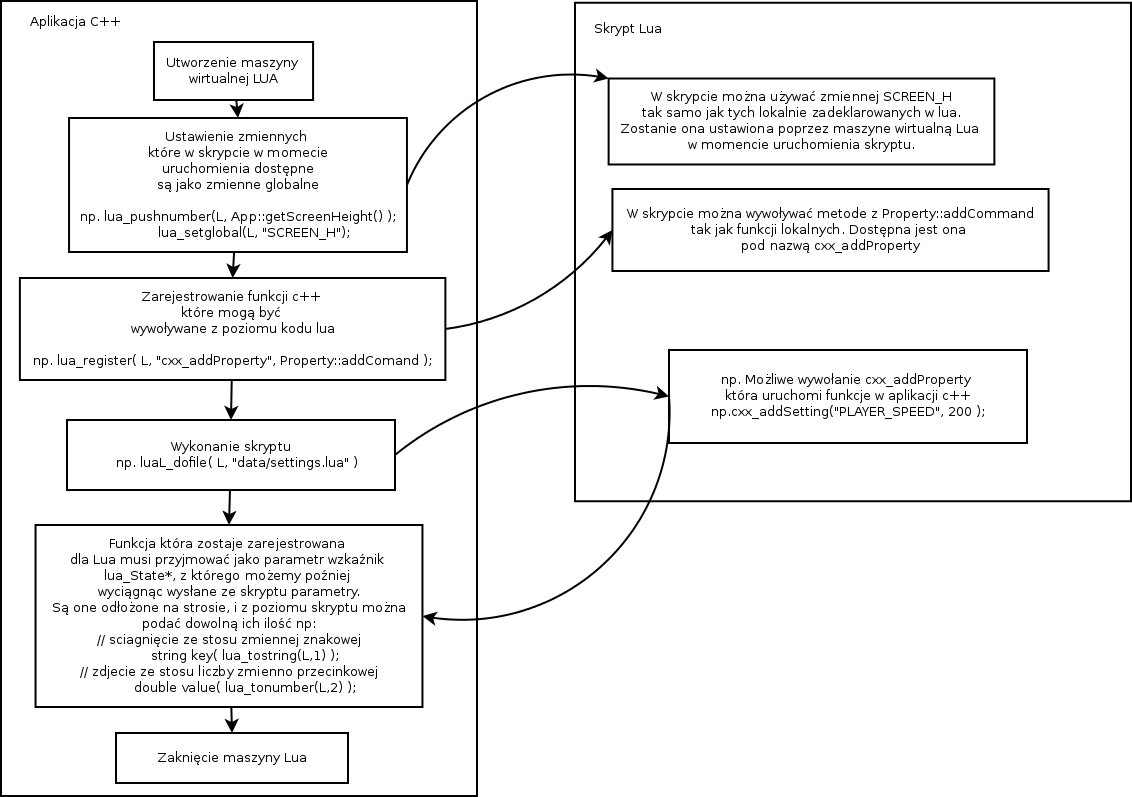
\includegraphics[width=0.8\textwidth,natwidth=410,natheight=142]{./Pictures/lua_skrypty.png}
    \caption{Przepływ danych między aplikacją C++ a skryptem Lua}
\end{figure}

Powyższy rysunek pokazuje przykładowy przepływ danych między aplikacją C++ a skryptem Lua. Wykorzystane tu zostało wywołanie funkcji C++ z poziomu skryptu, aczkolwiek w drugą stronę ten mechanizm również działa. To znaczy z poziomu C++ można wykonać funkcje Lua. Lua została wykorzystana do internacjonalizacji aplikacji. Podobnie jak to jest wykorzystywane w aplikacjach webowych w języku Java, gdzie wszystkie komunikaty są przechowywane w plikach properties. Podczas uruchamiania aplikacji zostaje odczytany odpowiedni plik dla danego języka. Cały proces ilustruje rysunek 5. W rezultacie takiej budowy aplikacja może działać z dowolnym językiem. Podczas tworzenia zostały napisane komunikaty zarówno polskie jak i angielskie.


%============================================================================================================================
%											Obsługa czcionek
%============================================================================================================================
\section{Obsługa czcionek w SDL}
\lhead{Rozdział 1. \emph{Obsługa czcionek w SDL}}
W projekcie została wykorzystana biblioteka SDL\_ttf pozwalająca używać w aplikacji czcionek w formacie True Type. Format ten stworzony przez firmę Apple przechowuje kształty poszczególnych liter jako krzywe Beziera, i jest on obsługiwany przez większość platform. Na Linuksie jest on bardzo powszechnym formatem do obsługi czcionek, dodatkowym plusem jest ogromna ilość czcionek na darmowych licencjach. W grze została wykorzystana czcionka "Ubuntu" udostępniona za darmo, i będąca domyślną czcionką w dystrybucji Linuksa o tej samem nazwie. Plik z taką czcionką (standardowo o rozszerzeniu *.ttf) jest wczytywany podczas uruchamiania aplikacji, następnie poprzez wywołania funkcji z biblioteki SDL\_ttf np. TTF\_RenderUTF\_Blended zostaje utworzona powierzchnia na której narysowany jest napis o podanej treści, kolorze oraz rozmiarze. 

Niestety powierzchnia taka jest zwracana jako wskaźnik na strukturę SDL\_Surface, przez co konieczna jest konwersja na format obsługiwany przez OpenGL-a. Niedogodność taka nie występowałaby gdyby do renderowania było wykorzystywane API biblioteki SDL. Identyczny problem występuje również przy renderowaniu innych elementów graficznych które są ładowane z dysku i zwracane jako SDL\_Surface* (Wczytywanie takie realizowane jest poprzez kolejną bibliotekę będącą uzupełnieniem SDL-a: SDL\_image. Służy ona do wczytywania plików graficznych w takich formatach jak np. JPEG, PNG, TIFF. W aplikacji wykorzystana jest tylko jedna funkcja 
z tej biblioteki stąd też nie będzie ona szerzej omawiana).

Sama konwersja SDL\_Surface* na GLuint to wygenerowanie tekstury w standardowy dla OpenGL-a sposób, wykorzystując przy tym pole pixels ze struktury SDL\_Surface, które jest adresem pod którym przechowywane są poszczególne piksele obrazka. W uproszczeniu funkcja realizująca taką konwersje w grze wygląda następująco:

\begingroup
\fontsize{10pt}{12pt}\selectfont
\begin{verbatim}  
void RendererGL::create_gl(SDL_Surface * surf, GLuint * tex )
{
 
   /** ...tutaj określenie ilości kolorów i formatu */
  
    glGenTextures( 1, tex );
    glBindTexture( GL_TEXTURE_2D, *tex );

    /** ...tutaj ustawienia parametrów tekstury */

    glTexImage2D( GL_TEXTURE_2D, 0, colors_amount,
    			  	surf->w, surf->h, 0, format, 
    			 	 GL_UNSIGNED_BYTE, surf->pixels );
}
\end{verbatim}
\endgroup

Warto wspomnieć że biblioteka SDL\_ttf pozwala renderować napisy z polskimi znakami, o ile takie występują w wczytanej czcionce. Ponadto SDL\_ttf dostępny jest podobnie jak SDL na darmowej licencji zlib, i jest wieloplatformowy jak wszystkie wtyczki do SDL-a. W niektórych dystrybucjach zainstalowanie tej biblioteki, oraz innych wspomnianych bibliotek rozszerzających SDL-a sprowadza się do wykonania jednego polecenia- zainstalowania pakietu z repozytorium. Dla dystrybucji Debian oraz jego pochodnych będzie to polecenie:
\begin{verbatim}
apt-get install libsdl-ttf2.0-dev 
\end{verbatim}
